\documentclass[aip,cha,reprint,a4paper,amsmath,amssymb]{revtex4-2}
\usepackage[utf8]{inputenc}
\usepackage[T2A]{fontenc}
\usepackage[english,russian]{babel}
\usepackage{bm}
\usepackage{graphicx}
\usepackage{hyperref}

\begin{document}

\title{Аналитическая теория встречного вращения двух заряженных частиц в двухчастотной электродинамической ловушке}
\author{Рабочая рукопись для обсуждения с Семёном}
\date{24 ноября 2026 г.}

\begin{abstract}
Исследуется встречное среднее вращение двух заряженных частиц в математической модели двухчастотного поперечного поля 24-электродной ловушки. Для ведущих бегущих пространственных гармоник $k=+2$ и $k=-4$ независимо выводятся радиальный корень, критический радиус нулевого медленного RF-момента и тождество, исключающее радиус. В слабодиссипативном пределе получено условие $\max\{1,\alpha_2(1+\nu)\}<\Pi<1+\nu$, где $\Pi=\beta/(4A^2)$, $\alpha_1=1$, $0<\alpha_2<1$. Оно строго предсказывает противоположные знаки нулевого медленного момента при положительном допустимом радиальном корне; для переноса к стационарным скоростям дополнительно требуются существование моментного корня и положительное эффективное угловое сопротивление. Номинальный параметрический набор лежит внутри полосы. M0 предсказание согласуется с 33 из 36 ранее опубликованных одномерных M3 точек; расхождения находятся у почти нулевой скорости первой частицы. Уже опубликованная полная RF динамика подтверждает номинальную встречную ветвь и выбранные режимы по обе стороны крупного изменения амплитуды, но не точную границу перехода. M3 Fourier-collocation оценка даёт медианные числа Reynolds 0.332 и 1.605. Парное M3 решение с/без Schiller--Naumann нелинейности сохраняет знаки частот, но изменяет их модули на 25.8\% и 11.1\%. Полученные результаты описывают аналитический механизм и проверенные численные ветви, но не доказывают притягивающий тор полной RF системы или физическую реализуемость конечной ловушки.
\end{abstract}

\maketitle

\noindent\textbf{Lead paragraph.} Два заряженных объекта в одном вращающемся электрическом поле могут получать противоположный угловой момент, если разные отношения заряда к массе сначала помещают их на разные радиусы, а конкурирующие бегущие гармоники меняют относительный вес как $r^2$ и $r^6$. Мы выводим открытое трёхпараметрическое условие для знаков момента в ограниченной ведущей модели, проверяем его на опубликованных M3 ветвях и показываем, что нелинейное сопротивление существенно меняет частоты, хотя сохраняет их знаки на номинальном режиме.


\section{Физическая задача и границы исследования}
В линейной идеализированной RF-ловушке обычно сначала рассматривают локализацию относительно оси: быстрое поле создаёт среднюю возвращающую силу, а дополнительное статическое поле определяет осевое положение. Здесь исследуется орбитальное движение другого типа. Две частицы в одном поле имеют разные средние радиусы и противоположные средние угловые скорости. Требуется объяснить, как одно внешнее возбуждение может одновременно передавать им угловой момент разных знаков.

Поле содержит два бегущих пространственных рисунка с противоположной киральностью. Их действие зависит от радиуса по разным степенным законам. Поэтому вопрос о направлении вращения нельзя отделить от вопроса о радиальной локализации. Сначала необходимо определить, на каком радиусе находится каждая частица, а затем сравнить моменты двух RF-семейств на этом радиусе. Именно эта последовательность позволяет исключить радиус из ведущего аналитического условия.

Мы рассматриваем поперечное поле бесконечно длинных цилиндрических электродов и отдельно заданный идеальный DC-квадруполь. Конечные торцы, поляризация диэлектриков, пробой и экспериментальная конструкция в эту модель не входят. Наблюдаемое движение является результатом численного решения определённых уравнений, а не экспериментальным измерением. На рис.~\ref{fig:geometry} схематически показан объект исследования. Две окружности означают средние орбиты; фактическая RF-траектория содержит микродвижение.

\begin{figure}[t]
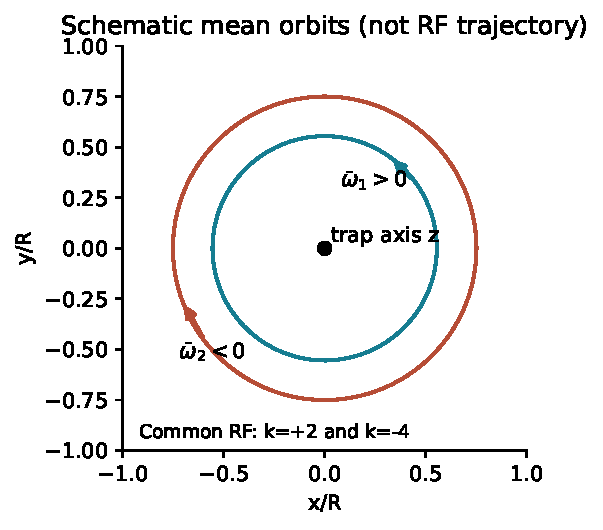
\includegraphics[width=\columnwidth]{figures/FIG01.pdf}
\caption{Geometry of the mean counterrotating motion. Schematic only: the circles are not stored RF trajectories. Both particles experience the same two RF families.}
\label{fig:geometry}
\end{figure}

\section{Уравнения и нормировка}
Для двух положительно заряженных частиц размерная система имеет вид
\begin{equation}
 m_i\ddot{\mathbf r}_i=q_i(\mathbf E_{\rm RF}+\mathbf E_{\rm DC})
 +\mathbf F_{C,i}+\mathbf F_{D,i}+m_i\mathbf g.
\end{equation}
Здесь $\mathbf F_{C,1}=q_1q_2(\mathbf r_1-\mathbf r_2)/(4\pi\varepsilon|\mathbf r_1-\mathbf r_2|^3)$, $\mathbf F_{C,2}=-\mathbf F_{C,1}$. Равенство сил не означает равенства ускорений. Радиус сферы далее обозначается $a_i$, чтобы отличать его от орбитального радиуса.

Введём $\boldsymbol\xi_i=\mathbf r_i/R$, $\tau=\Omega_1t$ и штрих как производную по $\tau$. Пусть $s=m_1/m_2$, $Q=q_2/q_1$ и $\alpha_i=(q_i/m_i)/(q_1/m_1)$: тогда $\alpha_1=1$, $\alpha_2=sQ$. Полная безразмерная система записывается компактно:
\begin{equation}\begin{split}
\boldsymbol\xi_i''={}&-\alpha_i\nabla_{\xi}\phi_{\rm RF}
+\alpha_i\beta(x_i,y_i,-2z_i)\\
&+\epsilon_i\mu_i C_{12}\frac{\mathbf d}{|\mathbf d|^3}
-\lambda_i[1+0.15(Re_{*,i}|\boldsymbol\xi_i'|)^{0.687}]
\boldsymbol\xi_i'+\mathbf g_*,
\end{split}\end{equation}
где $\mathbf d=\boldsymbol\xi_1-\boldsymbol\xi_2$, $(\epsilon_1,\epsilon_2)=(1,-1)$, $(\mu_1,\mu_2)=(1,s)$ и $\mathbf g_*=\mathbf g/(R\Omega_1^2)$. В каждом уравнении ускорение нормировано на $R\Omega_1^2$.

Стоксов коэффициент с принятой поправкой скольжения равен $\lambda_i=6\pi\eta a_i/(C_{c,i}m_i\Omega_1)$; $C_c$ делит сопротивление. Диаметральное число Рейнольдса есть $Re_i=Re_{*,i}|\boldsymbol\xi_i'|$, где $Re_{*,i}=2\rho_f a_iR\Omega_1/\eta$. Скорость включает RF-микродвижение. Кулоновская нормировка:
\begin{equation}
 C_{12}=\frac{q_1q_2}{4\pi\varepsilon m_1R^3\Omega_1^2}.
\end{equation}
Коэффициент второй частицы равен $sC_{12}$, что обеспечивает сохранение полного механического импульса внутренними силами в размерной системе.

Для $w=x+iy$ потенциал восьмигармонического MFS-представления имеет вид
\begin{equation}\begin{split}
\phi_{\rm RF}={\rm Re}\{&A e^{-i\psi_1}\sum_{k\in H_1}c_kw_k^{|k|}\\
 &+B e^{-i\psi_2}\sum_{k\in H_2}c_kw_k^{|k|}\},
\end{split}\end{equation}
где $w_k=w$ при $k>0$, $w_k=\bar w$ при $k<0$,
$H_1=\{-46,-22,2,26\}$, $H_2=\{-28,-4,20,44\}$,
$\psi_1=\tau+\psi_{10}$, $\psi_2=\nu\tau+\psi_{20}$.
Коэффициенты $c_k$ комплексны и заданы электростатическим решением; $c_2=c_{-4}=1$ в принятой ведущей нормировке. Умножение на $A$ или $B$ масштабирует всё соответствующее семейство.

Амплитуды $A,B$ относятся к ведущим потенциалам, а не непосредственно к электродным напряжениям. Если $h_1,h_2$ являются transfer factors из напряжения в ведущую гармонику, то
\begin{equation}\begin{aligned}
 A&=\frac{q_1h_1U_1}{m_1R^2\Omega_1^2},&
 B&=\frac{q_1h_2U_2}{m_1R^2\Omega_1^2},\\
 \nu&=\Omega_2/\Omega_1,&
 \beta&=\frac{2q_1V_2}{m_1R^2\Omega_1^2}.
\end{aligned}\end{equation}
Последняя формула следует из $\Phi_{\rm DC}=V_2(z^2-\rho^2/2)/R^2$. Все коэффициенты безразмерны. Положительное $\beta$ удерживает положительные заряды по оси и расталкивает их от оси в поперечной плоскости.

Номинальные значения составляют $A=0.0349241328240$, $B=0.156316673329$, $\nu=3.219677363802$, $\beta=0.0153885591405$, $s=0.109637639065$, $C_{12}=9.74726545686\cdot10^{-6}$, $\alpha_2=0.378146096180$. Коэффициенты сопротивления равны $0.244523071231$ и $0.177365987311$; $Re_{*,i}=6.64373,43.76776$. Численные данные ниже относятся к одному этому набору либо к явно указанным изменениям поля при фиксированных частицах.

\section{Радиальная локализация}
Разделим движение на среднюю орбиту $\mathbf R_i$ и RF-микродвижение $\boldsymbol\eta_i$. В ведущей оценке средняя угловая скорость принимается нулевой при вычислении быстрого отклика. Удерживаются моды $+2,-4$, линейное сопротивление и DC-якобиан; Coulomb, центробежное ускорение и средний радиальный drag в этом балансе опущены.

Линейная восприимчивость содержит
\begin{equation}\begin{aligned}
K_{1i}&=1+\alpha_i\beta,& K_{2i}&=\nu^2+\alpha_i\beta,\\
D_{1i}&=K_{1i}^2+\lambda_i^2,&
D_{2i}&=K_{2i}^2+(\lambda_i\nu)^2.
\end{aligned}\end{equation}
Члены $\alpha_i\beta$ сохраняют воздействие DC-поля на быстрый ответ. Усреднённая радиальная сила имеет вид
\begin{equation}\begin{split}
0={}&\alpha_i\beta r_i
-\frac{4\alpha_i^2A^2|c_2|^2K_{1i}}{D_{1i}}r_i\\
&-\frac{48\alpha_i^2B^2|c_{-4}|^2K_{2i}}{D_{2i}}r_i^5.
\end{split}\label{eq:rad}\end{equation}
Здесь и далее $r_i$ уже нормирован на $R$. Радиальная RF-реакция возникает как среднее произведение градиента поля на смещение: поле создаёт смещение первого порядка по $\alpha_i$, а умножение на заряд в уравнении силы даёт второй множитель $\alpha_i$. Напротив, DC-ускорение непосредственно пропорционально $\alpha_i$. Это различие объясняет сортировку частиц по радиусу.

Обозначим
\begin{equation}\begin{aligned}
U_i&=\alpha_i\beta-\frac{4\alpha_i^2A^2|c_2|^2K_{1i}}{D_{1i}},\\
V_i&=\frac{48\alpha_i^2B^2|c_{-4}|^2K_{2i}}{D_{2i}}.
\end{aligned}\end{equation}
После деления (\ref{eq:rad}) на ненулевой $r_i$ получается $U_i-V_ir_i^4=0$, откуда
\begin{equation}r_i^4=U_i/V_i.\label{eq:root}\end{equation}
В нашей области $V_i>0$, поэтому положительный корень требует $U_i>0$. При произвольных знаках формальный критерий есть $U_i/V_i>0$, но отрицательные $U_i,V_i$ дают невозвращающий наклон и не относятся к рабочему режиму. Для $U_i,V_i>0$ производная радиальной силы в корне равна $U_i-5V_ir_i^4=-4U_i<0$. Это локальный возвращающий наклон при фиксированном нулевом спине, а не доказательство устойчивости связанной системы.

В пределе малых $\lambda_i,\alpha_i\beta$ имеем $r_i^4\simeq\nu^2(\beta/\alpha_i-4A^2)/(48B^2)$. Поэтому меньшая $\alpha_i$ при прочих равных даёт больший радиус. При конечных коэффициентах восприимчивость также зависит от вида частицы; монотонность нельзя объявлять общей теоремой для всех параметров.

В номинале ведущие радиусы равны $0.557449R,0.751674R$, полная RF-траектория даёт $0.555721R,0.751516R$. Относительные расхождения составляют $0.311\%$ и $0.0211\%$. Рис.~\ref{fig:rad} показывает именно силы ведущего приближения. Малость ошибки здесь не переносится автоматически на другие параметры. Дополнительно нужны апертура $r_i+a_i/R<r_{\rm ap}/R$, отсутствие контактов и контролируемое микродвижение.

\begin{figure*}[t]
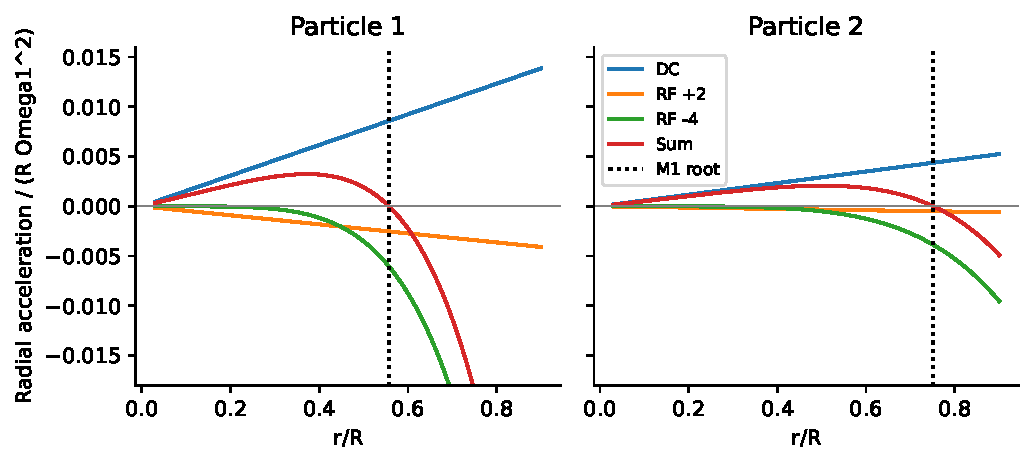
\includegraphics[width=.94\textwidth]{figures/FIG02.pdf}
\caption{Radial acceleration balance at nominal parameters in the zero-orbit-speed leading model (M1). The DC term is outward, both RF terms are inward. Dotted lines mark M1 roots; full-RF reference radii are compared in Fig.~5.}
\label{fig:rad}\end{figure*}

\section{Передача углового момента}
Осевой момент размерной силы равен $M_z=(\mathbf r\times\mathbf F)_z$. В безразмерном уравнении частицы он нормируется на $m_iR^2\Omega_1^2$; угловой момент нормируется на $m_iR^2\Omega_1$. Поэтому суммы моментов разных частиц требуют возврата к общей массовой нормировке.

Для одной гармоники положим $n=|k|$, $\sigma=\operatorname{sgn}k$, $\nu_j=1$ либо $\nu$. Угловая зависимость потенциала есть $\cos(k\theta-\psi_j+\arg c_k)$, так что знак $k$ определяет направление бегущего рисунка при положительной временной частоте. Прямой фазовый ответ определяется комплексным знаменателем $K+i\lambda\nu_j$ (знак мнимой части зависит от Fourier-конвенции). Его модуль в квадрате $D=K^2+(\lambda\nu_j)^2$. Именно диссипативная квадратура, пропорциональная $\lambda\nu_j/D$, даёт ненулевой средний момент. При отсутствии фазового запаздывания ведущая инжекция момента исчезает.

Введём $P=\alpha^2n^2|a_jc_k|^2r^{2n-2}$, где $a_1=A,a_2=B$. Амплитуда кругового микродвижения в квадрате равна $P/D$, а его средний угловой момент:
\begin{equation}\bar L_{\rm micro}=\sigma P\nu_j/D.\end{equation}
При раскрытии $\langle(\mathbf R+\boldsymbol\eta)\times\mathbf F_{\rm RF}\rangle$ слагаемое $\langle\boldsymbol\eta\times\mathbf F_{\rm RF}\rangle$ даёт момент микродвижения. Второе слагаемое получается из изменения силы на смещении, $\mathbf R\times\langle(\boldsymbol\eta\cdot\nabla)\mathbf F_{\rm RF}\rangle$; однородность силы степени $n-1$ даёт множитель $n-1$. Таким образом,
\begin{equation}\begin{aligned}
\bar M_{\rm RF,micro}&=\sigma P\lambda\nu_j/D,\\
\bar M_{\rm RF,orbit}&=\sigma(n-1)P\lambda\nu_j/D,\\
\bar M_{\rm RF,total}&=\sigma nP\lambda\nu_j/D.
\end{aligned}\end{equation}
При линейном drag $\bar M_{D,\rm micro}=-\lambda\bar L_{\rm micro}$ точно компенсирует первую строку в этом порядке. Для медленной орбиты остаётся вторая строка. Следовательно, нуль полного RF-момента и нуль эффективного медленного момента различны. Под моментом микродвижения здесь понимается средняя передача силы быстрому движению; он не тождественен самому угловому моменту $L_{\rm micro}$.

Для $+2$ медленная передача пропорциональна $+4\alpha^2A^2\lambda r^2/D_1$, для $-4$ она равна $-48\alpha^2B^2\lambda\nu r^6/D_2$. Их отношение по модулю растёт как $r^4$. Полные RF-моменты имеют вместо коэффициентов $4,48$ коэффициенты $8,64$. На рис.~\ref{fig:torque} эти разные величины показаны раздельно.

\begin{figure*}[t]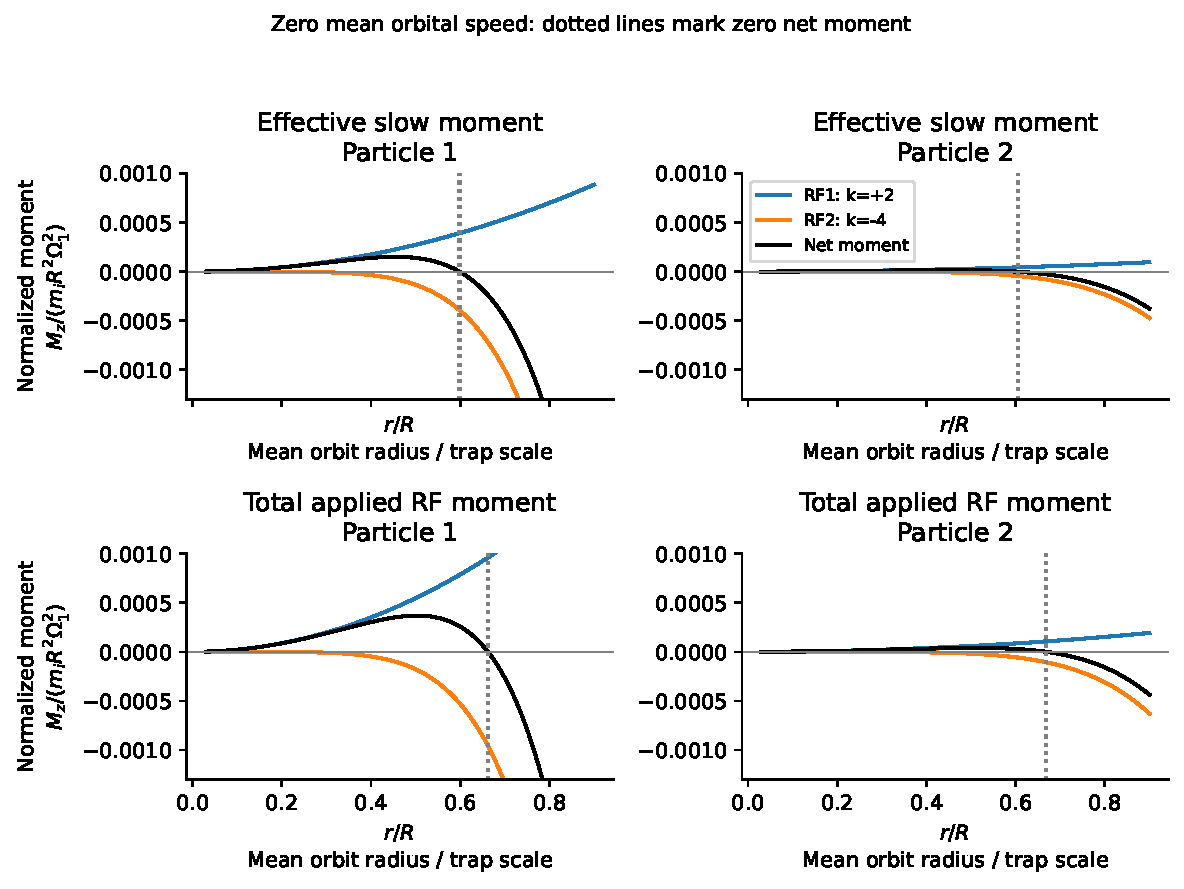
\includegraphics[width=.94\textwidth]{figures/FIG03.pdf}
\caption{Competition of the two leading traveling modes at zero mean orbital speed. Top: net torque available to the slow orbit after micromotion drag. Bottom: total RF torque. These are different observables with different zero radii. All curves use nominal finite damping and DC susceptibility.}
\label{fig:torque}\end{figure*}

Полное M3-замыкание на одной и той же микродвигательной орбите даёт для частицы~1 моменты RF1 $+7.5171\cdot10^{-4}$ и RF2 $-3.6499\cdot10^{-4}$; их сумма $+3.8672\cdot10^{-4}$ компенсируется drag. Для частицы~2 получены $+1.6793\cdot10^{-4}$ и $-2.6012\cdot10^{-4}$; сумма $-9.2189\cdot10^{-5}$ также компенсируется drag. Это полные RF-моменты, а не две ведущие кривые верхней панели. Разложение по семействам выполнено на общем полном решении, а не сложением независимо рассчитанных одночастотных орбит.

\section{Исключение радиуса и трёхпараметрическое условие}
Суммарный медленный момент при нулевом спине:
\begin{equation}\begin{split}
\mathcal T_i(0)={}&\frac{4\alpha_i^2A^2|c_2|^2\lambda_i}{D_{1i}}r_i^2\\
&-\frac{48\alpha_i^2B^2|c_{-4}|^2\lambda_i\nu}{D_{2i}}r_i^6.
\end{split}\end{equation}
При $r_i>0$, $\lambda_i>0$ вынесем положительный первый коэффициент. Знак суммы совпадает со знаком $1-S_i$, где
\begin{equation}\begin{aligned}
r_{{\rm cr},i}^4&=\frac{A^2|c_2|^2D_{2i}}{12B^2|c_{-4}|^2\nu D_{1i}},\\
S_i&=r_i^4/r_{{\rm cr},i}^4.
\end{aligned}\end{equation}
Подставим (\ref{eq:root}) без пропуска сокращений:
\begin{equation}\begin{split}
S_i={}&\left(\alpha_i\beta-
\frac{4\alpha_i^2A^2|c_2|^2K_{1i}}{D_{1i}}\right)\\
&\times\frac{D_{2i}}{48\alpha_i^2B^2|c_{-4}|^2K_{2i}}
\frac{12B^2|c_{-4}|^2\nu D_{1i}}{A^2|c_2|^2D_{2i}}\\
={}&\frac{\nu}{K_{2i}}\left[
\frac{\beta D_{1i}}{4\alpha_iA^2|c_2|^2}-K_{1i}\right].
\end{split}\label{eq:S}\end{equation}
Сократились $D_{2i}$ и $B^2|c_{-4}|^2$. Это алгебраическое следствие общей степенной зависимости радиальной силы и момента моды $-4$, а не исчезновение физической роли RF2. Радиус остаётся пропорциональным $B^{-1/2}$, так что уменьшение $B$ может вывести орбиту за апертуру. Предел $B=0$ сингулярен. Исключение стационарного радиуса также не исключает радиальное возмущение из динамической системы.

Для $|c_2|=|c_{-4}|=1$, $\lambda_i^2\ll1$, $|\alpha_i\beta|\ll1$ и $|\alpha_i\beta|\ll\nu^2$:
\begin{equation}
 S_i\simeq\frac{\Pi/\alpha_i-1}{\nu},\qquad
 \Pi=\frac{\beta}{4A^2}.
\end{equation}
Это предел малой положительной диссипации: при строго $\lambda=0$ сам момент равен нулю, и знаковое утверждение не переносится на недиссипативную систему.

Положительный радиус частицы~1 требует $\Pi>1$, а её положительный момент требует $S_1<1$, то есть $\Pi<1+\nu$. Для частицы~2 отрицательный момент требует $S_2>1$, то есть $\Pi>\alpha_2(1+\nu)$. Последнее автоматически сильнее условия её положительного радиуса $\Pi>\alpha_2$ при $\nu>0$. Пересечение даёт
\begin{equation}
\boxed{\max\{1,\alpha_2(1+\nu)\}<\Pi<1+\nu.}
\end{equation}
Равенство верхней границе означает нулевой момент первой частицы; нижняя граница либо отвечает исчезновению ненулевого радиального корня первой частицы, либо нулевому моменту второй. При $|c_2|\ne1$ вместо $\Pi$ нужно использовать $\beta/(4A^2|c_2|^2)$.

Получено условие знаков $\mathcal T_i(0)$ в ведущем приближении. Для стационарных скоростей дополнительно нужен корень полного момента $\mathcal T_i(\omega_i)=0$. Локальное приближение $\omega_i\simeq\mathcal T_i(0)/D_i^{\rm eff}$ допустимо при $D_i^{\rm eff}=-\partial_{\omega_i}\mathcal T_i>0$ и контролируемой линейности. Положительный наклон эффективного сопротивления и существование корня нельзя выводить из одного неравенства, особенно около нулевой скорости.

\begin{figure*}[t]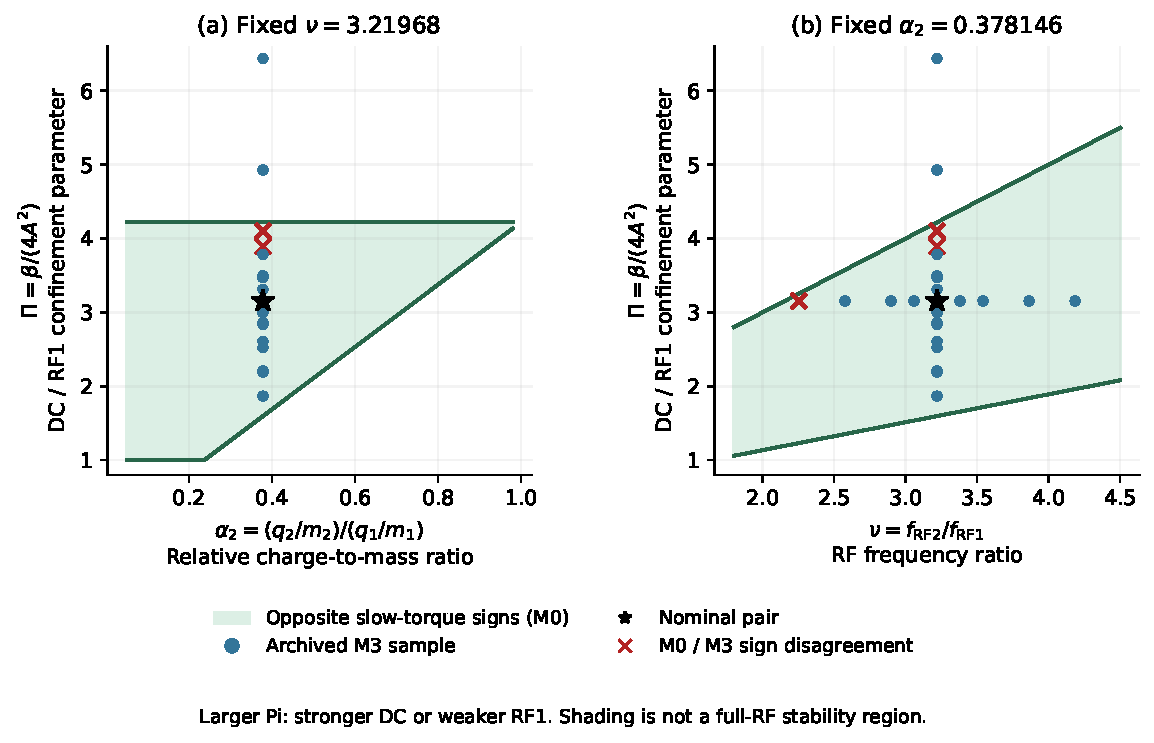
\includegraphics[width=.94\textwidth]{figures/FIG04.pdf}
\caption{Three-parameter leading criterion. The vertical parameter $\Pi=\beta/(4A^2)$ compares DC defocusing with the RF1 confinement scale. Panel (a): relative charge-to-mass ratio at fixed $\nu=3.21968$. Panel (b): RF frequency ratio at fixed $\alpha_2=0.378146$. Shading denotes opposite zero-speed slow torque signs in M0, not full-RF stability. Dots reuse archived M3 branch samples; red crosses identify all three M0/M3 sign disagreements. No interpolation of a numerical stability boundary is implied.}
\label{fig:criterion}\end{figure*}

На рис.~\ref{fig:criterion} вертикальная координата $\Pi$ характеризует отношение DC-выталкивания к масштабу RF1-удержания: она растёт при усилении DC или ослаблении первой RF-компоненты. Частотное отношение $\nu=f_{\rm RF2}/f_{\rm RF1}$ показывает, во сколько раз второе возбуждение быстрее первого. Слева изменяется относительное отношение заряда к массе $\alpha_2$ при фиксированном $\nu=3.21968$; справа изменяется $\nu$ при фиксированном $\alpha_2=0.378146$. Зелёная полоса обозначает противоположные знаки ведущих медленных моментов, а не установленную область устойчивости полной системы.

\section{Сопоставление с численными расчётами}
В дальнейшем M0 означает слабодиссипативное неравенство; M1 сохраняет конечные $\lambda_i$ и DC в ведущих формулах; M2 учитывает движение орбиты в быстром отклике; M3 сохраняет все восемь гармоник и нелинейный drag через Fourier-collocation. Полная RF-система интегрирует все 12 механических координат без замены быстрых сил их средними. Это разные уровни приближения, а не независимые эксперименты.

В номинале $\Pi=3.1541817$ и $\alpha_2(1+\nu)=1.5956545$, тогда как $1+\nu=4.2196774$. Точка находится внутри полосы. M0 даёт $S_1=0.66907,S_2=2.28010$; M1 даёт $0.75213,2.38869$. Поправка заметна прежде всего для внутренней орбиты. Поэтому геометрический запас до перехода нельзя оценивать только по M0.

В ограниченной выборке 36 ранее сохранённых точек продолжения M3 получено согласие знаков в 33 случаях при пороге нулевой скорости $10^{-5}\Omega_1$. Три расхождения относятся к $A=0.9A_0$, $\nu=0.7\nu_0$ и $\beta=1.3\beta_0$. Все они близки к смене направления частицы~1. Это проверка на выбранной ветви, а не универсальная оценка точности и не случайная независимая выборка параметров. Рис.~\ref{fig:criterion} показывает также точку расхождения при изменённой $\nu$, которую нельзя помещать на номинальный частотный срез.

Полная опубликованная RF-проверка включает 7 интегрирований, суммарно 116000 RF1-периодов и 7.904 млн шагов RK4. Номинал и $A=0.95A_0$ дали встречное вращение, $A=0.8A_0$ дал два отрицательных знака. При уменьшении $A$ параметр $\Pi$ увеличивается как $A^{-2}$, что согласуется с выходом через верхнюю границу M0. Непосредственно у предполагаемого перехода первая частица совершила только $-0.093$ либо $+0.022$ оборота; такие случаи остаются неразрешёнными. При $\beta=1.3\beta_0$ около пяти оборотов также не удовлетворяют принятому ориентиру десяти оборотов. Точное положение границы полной системы этими данными не установлено.

Архивная длинная номинальная траектория содержит 240000 RF1-периодов и даёт $f_1=+0.0546477$ Гц, $f_2=-0.0484539$ Гц. M3 предсказывает $+0.0547223,-0.0487398$ Гц при радиусах $0.5550375R,0.7513383R$. Радиусы сопоставлены на рис.~\ref{fig:comparison}. В используемом размерном масштабе RF1 равна 50 Гц, поэтому $\omega/\Omega_1=f_{\rm orb}/50\,\mathrm{Hz}$. Размерные частоты здесь лишь восстанавливают масштаб архивного benchmark.

Численная сходимость Fourier-решения и точность усреднённой модели различаются. Для разложения моментов на сетке $192\times16\times16$ относительные внутренние невязки составляют $4.08\cdot10^{-9}$ и $1.60\cdot10^{-10}$; это малая ошибка решения дискретизированной задачи. Она не ограничивает погрешность адиабатического усреднения. Аналогично шаговое сравнение RK4 с 64 и 96 шагами на RF1-период и архивные проверки DOP853 контролируют интегрирование выбранной модели, но не её полноту как описания реальной жидкости или газа.

\section{Reynolds и роль диссипации}
Перенормировка скорости на Reynolds может заменить $|\boldsymbol\xi_i'|$ на $Re_i$, но при этом коэффициенты сил приобретают множители $Re_{*,i}$. Она не устраняет размеры, вязкость и плотность среды из полной системы. В частности, две частицы имеют разные $Re_{*,i}$, и единая замена переменной не делает их сопротивления одинаковыми.

На фазовой сетке M3 с учётом полной скорости медианные $Re_i$ равны $0.332$ и $1.605$, максимальные $0.505$ и $2.279$. Это статистика узлов замыкания, а не независимая статистика RF-траектории. Средние множители Schiller--Naumann равны $1.0640$ и $1.1944$. Умножение средней скорости на средний drag-фактор не заменяет усреднения нелинейного произведения: скорость и множитель коррелированы через микродвижение.

В парном повторном решении M3 на общей сетке $96\times8\times8$ с удвоенной квадратурой нелинейный drag даёт $+0.0547222,-0.0487402$ Гц; линейный контроль даёт $+0.0405961,-0.0433507$ Гц. Разности модулей относительно нелинейного решения равны $25.8\%$ и $11.1\%$. Радиусы меняются лишь на $0.134\%$ и $0.092\%$. Следовательно, радиальная локализация менее чувствительна к этой замене, чем малый остаток конкурирующих моментов. Знак может сохраняться благодаря запасу до смены направления, хотя частота существенно изменяется. Это не оправдывает пренебрежение нелинейностью для количественного прогноза.

\begin{figure*}[t]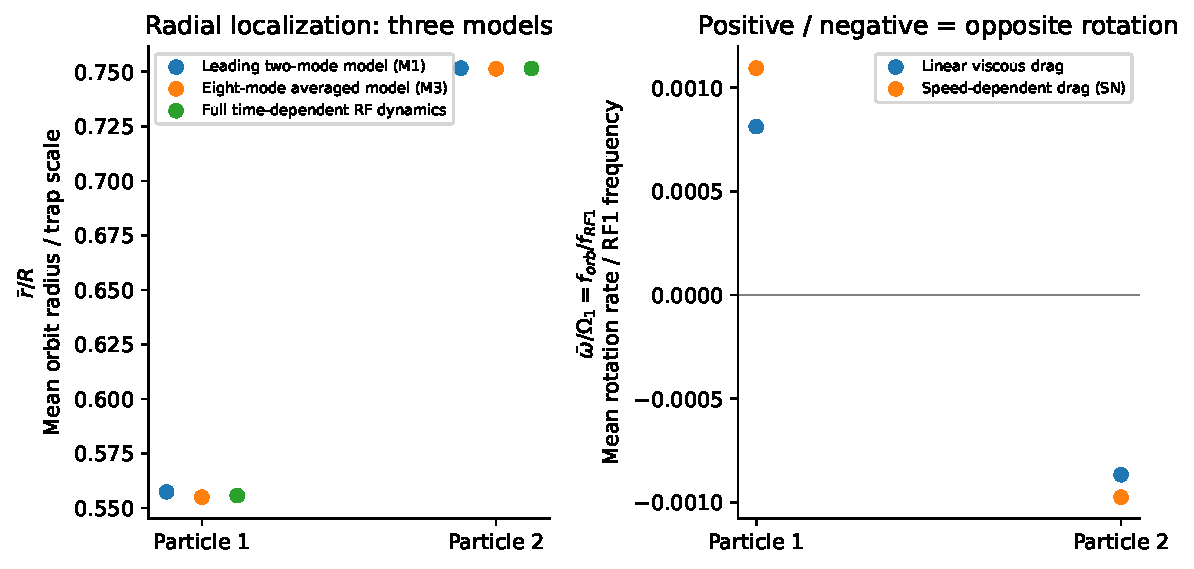
\includegraphics[width=.94\textwidth]{figures/FIG05.pdf}
\caption{Nominal analytical and numerical comparison. Left: leading finite-damping radius, M3 and archived full-RF means. Right: paired M3 roots with nonlinear Schiller--Naumann and linear drag at identical collocation settings. No connecting curve or statistical uncertainty is inferred from these discrete results.}
\label{fig:comparison}\end{figure*}

Выбранная корреляция сопротивления входит в математическую модель; её использование само по себе не проверяет нестационарную гидродинамику, силу памяти, поляризацию или влияние стенок. Данные о численной точности нельзя переносить на физическую точность сопротивления без отдельного анализа этих эффектов.

\section{Физическая интерпретация и устойчивость}
Механизм складывается из двух последовательных процессов. Различие $q/m$ меняет баланс линейного по $\alpha$ DC-выталкивания и квадратичного RF-удержания. Частицы занимают разные средние радиусы. На внутренней орбите сильнее положительная передача первой бегущей гармоники; на внешней возрастает относительный вес отрицательной передачи второй. Сопротивление ограничивает скорость, а RF-питание непрерывно восполняет диссипируемый момент и энергию. Это вынужденное диссипативное состояние; принцип минимизации полного механического углового момента к нему неприменим.

Кулоновские силы перераспределяют момент между частицами и меняют их относительную динамику. Суммарный размерный внутренний момент центральных парных сил равен нулю. На проверенном старте встречное вращение сохранялось и при $C_{12}=0$, поэтому взаимодействие не является необходимым источником знаков. Оно может влиять на фазовые связи, расстояния и устойчивость, но эти эффекты требуют самостоятельных свидетельств.

Об орбитальной киральности можно говорить как о знаке среднего обхода вокруг общей оси. Два противоположных знака не означают кристаллического порядка. Для термина <<кулоновский кристалл>> потребовались бы установленные устойчивые взаимные положения в соответствующих движущихся координатах и анализ внутренних мод. Две вращающиеся частицы с изменяющейся относительной фазой сами по себе такого порядка не доказывают.

Осесимметричное усреднение также не означает мгновенной осевой симметрии поля. Потенциал содержит дискретные пространственные гармоники и две внешние фазы. В квазипериодическом возбуждении стробоскопия по RF1 не возвращает RF2-фазу, поэтому нельзя автоматически применять периодическую теорию Флоке.

Существование алгебраического корня, его локальная устойчивость в M3 и притяжение полной системы являются разными утверждениями. В адиабатическом M3-потоке получены десять собственных значений с отрицательными действительными частями. Но этот поток исключает быстрый ответ квазистационарно. В полной RF-системе два механических условных показателя близки к нулю, остальные существенно отрицательны. Без надёжной идентификации касательных направлений и геометрии инвариантного множества нельзя объявить два первых направления доказанными фазами тора, а остальные автоматически поперечными. Длительное удержание и сохранение знаков совместимы с притягивающим тором, слабым сжатием или квазинейтральной динамикой; они не выбирают единственную альтернативу.

Наиболее сильный вывод имеющихся данных: долгоживущее встречное вращение в полной заданной RF-модели и локально устойчивый корень отдельной усреднённой модели. Полный притягивающий инвариантный тор не доказан. Для усиления вывода потребуются контроль геометрии множества, сжатия поперечных возмущений при сохранённых внешних фазах и сходимости показателей по горизонту.

\section{Выводы}
Радиальное исключение даёт компактное неравенство в трёх параметрах, поскольку одинаковый множитель второй гармоники входит в радиальную локализацию и медленный момент. Это условие противоположных знаков нулевого медленного момента в ведущем приближении. Оно объясняет номинальный режим и согласуется с большей частью сохранённых M3-точек; расхождения около смены знака показывают предел его прямого переноса на конечную скорость. Полная динамика подтверждает выбранные встречные и совместные режимы, но точная граница и притягивающий характер остаются неустановленными. Нелинейное сопротивление необходимо для количественного описания частот даже при сохранении качественного знакового механизма.

\section{Вопросы для научного обсуждения}
\begin{enumerate}
\item Достаточно ли обосновано исключение радиуса из ведущего критерия и какие его пределы наиболее опасны: малая RF2-амплитуда, апертура или нарушение малого микродвижения?
\item Можно ли получить более строгий критерий знака стационарной скорости без предположения о малом $\omega$, контролируя монотонность полного момента?
\item Насколько обоснована интерпретация через конкуренцию RF-моментов и радиальную локализацию при сохранении высших гармоник и нелинейного сопротивления?
\item Какие дополнительные условия нужны для перехода от долгоживущего встречного движения к утверждению об устойчивом коллективном орбитальном состоянии?
\end{enumerate}

\begin{thebibliography}{2}
\bibitem{archive} Counterrotating Motion, архив исходных уравнений, численных данных и M3-замыкания, \url{https://github.com/snejokzboxik/counterrotating-motion}. Зафиксированный исходный коммит: \texttt{4f8232b8}; детальные источники и контрольные суммы включены в сопроводительный пакет.
\bibitem{method} Архивные научные материалы: полная динамика V17C.20B, гармонический баланс V17C.21A и продолжение V17C.21B. Их определения и численные результаты использованы без изменения физических параметров и без новых массовых интегрирований.
\end{thebibliography}
\end{document}
